Questa sezione descrive il processo di sviluppo adottato nell'ambito del profetto \emph{GoBus}.

\subsection{Modello del Ciclo di Vita}
In base alle esigenze relative alle tempistiche e agli obiettivi del progetto, il modello del ciclo di vita che meglio si adatta \`{e} il ciclo \emph{evolutivo a prototipazione}. In particolare, vista la necessita di comprendere meglio i requisiti che il committente richiedeva, la tecnica utilizzata consente di fornirgli un prototipo del sistema in tempi rapidi. In questo modo, \`{e} possibile periodicamente avere feedback utili per la continuazione delle attivit\`{a} progettuali.

\subsection{Requirement Elicitation and Analysis}
La fase di requirement elicitation consiste nella comprensione delle necessit\`{a} del committente, al fine di collezionare i requisiti del sistema. Nell'ambito del progetto, tale attivit\`{a} \`{e} stata svolta facendo brainstorming con tutti gli stakeholder interessati. In particolare, sono stati organizzati incontri sia con i coordinatori del progetto sia con aziende di trasporto locali. Per mitigare il richio di errata comprensione delle reali necessit\`{a} degli stakeholder, i meeting si sono ripetuti così che, ad ogni incontro, i requisiti potessero essere meglio fissati. Il numero totale di incontri con gli stakeholder \`{e} 3.\\
La tabella \ref{tab:gestioni} mostra, ad alto livello, i principali raggruppamenti delle funzionalità identificate nell'ambito del progetto \emph{GoBus}. Di seguito verr\`{a} analizzato in dettaglio ciascun raggruppamento. Si noti che per evitare ridondanza e per ragioni di spazio, non sono riportati tutti i requisiti funzionali identificati. Per la lista completa, si faccia riferimento al Documento di Analisi dei Requisiti (RAD) in allegato.\\

\begin{table*}[tb]
   \centering
   \caption{Overview delle Funzionalit\`{a} Identificate}
   \label{tab:gestioni}
  \resizebox{1\linewidth}{!}{
   \begin{tabular}{ll}\hline
   Nome & Descrizione\\\hline
   Gestione Registrazione & Insieme di funzionalit\`{a} che consentono la registrazione di un nuovo utente.\\
   Gestione Autenticazione & Insieme di funzionalit\`{a} che consente il riconoscimento degli utenti registrati.\\
   Gestione Account & Insieme di funzionalit\`{a} per la manipolazione degli account degli utenti.\\
   Gestione Fermate & Funzionalit\`{a} che consente di visualizzare le fermate tramite l’applicazione di diversi filtri per la ricerca mirata.\\
   Gestione Linee & Funzionalit\`{a} che consente la visualizzazione delle linee tramite l’applicazione di diversi filtri per la ricerca mirata.\\
   Gestione Percorso & Insieme di funzionalit\`{a} che consente la visualizzazione delle indicazioni stradali.\\
   Gestione Preferiti & Funzionalit\`{a} che consente la gestione delle fermate e delle linee preferite.\\
   Gestione News & Insieme di funzionalit\`{a} per la efficace gestione degli avvisi da parte delle aziende di trasporti.\\
   Gestione Dati GTFS & Insieme di funzionalit\`{a} che consente ad un’azienda di trasporti di caricare il proprio file GTFS.\\
   \hline
   \end{tabular}
   }
\end{table*}

\noindent {\bf{Gestione Registrazione}}: La gestione della registrazione da la possibilità ad un nuovo utente di potersi iscrivere alla piattaforma. Vale la pena notare che la registrazione è consentita i) utilizzando la propria e-mail, fornendo un nickname ed una password; ii) tramite l'utilizzo dell'account Facebook; iii) tramite l'utilizzo dell'account Google. Questo insieme di requisiti \`{e} comune sia alla parte relativa alla web application che all'applicazione mobile.
\noindent {\bf{Gestione Autenticazione}}: Questa gestione permette ad un utente registrato di essere riconosciuto e abilitato a effettuare determinate operazioni da parte del sistema. Quindi, le funzionalit\`{a} di login e logout fanno parte di questa gestione.\\

\noindent {\bf{Gestione Account}}: Questo insieme di funzionalit\`{a} si occupa di tutto ciò che ha a che fare con la manipolazione delle informazioni personali degli utenti registrati al sistema. Nel dettaglio, \`{e} possibile visualizzare, modificare ed eliminare un account dalla piattaforma.\\

\noindent {\bf{Gestione Fermate}}: Questa funzionalit\`{a} permette di visualizzare le fermate tramite l’applicazione di diversi filtri, al fine di effettuare una ricerca mirata delle informazioni di cui l’utente necessita. I requisiti funzionali identificati riguardano la visualizzazione delle fermate tramite i) geo-localizzazione della posizione dell'utente; ii) una localit\`{a} specifica; o iii) nome della localit\`{a}. Inoltre, \`{e} possibile visualizzare le linee relative ad una fermata, consentendo quindi di conoscere, data una fermata, quali linee la percorrono.\\

\noindent {\bf{Gestione Linee}}: Questa funzionalit\`{a} permette di visualizzare le linee tramite l’applicazione di diversi filtri per effettuare una ricerca mirata delle informazioni di cui l’utente necessita. Sar\`{a} consentita la visualizzazione delle: linee di una specifica localit\`{a}, ma anche la ricerca di una linea e la visualizzazione di tutte le corse di una linea con i relativi orari di andata e ritorno. Inoltre, sar\`{a} implementata anche la visualizzazione dell'intero percorso di una determinata corsa.\\

\noindent {\bf{Gestione Percorso}}: Questa funzionalit\`{a} da all'utente la possibilit\`{a} di richiedere la navigazione tra un punto di partenza ed uno di arrivo.\\

\noindent {\bf{Gestione Preferiti}}: Tramite questa funzionalit\`{a} l'utente avr\`{a} la possibilit\`{a} di memorizzare le sue corse, linee, e citt\`{a} preferite, cos\`{i} da poter rapidamente accedere a tali informazioni in futuro.\\

\noindent {\bf{Gestione News}}: Questa funzionalit\`{a} è implementata esclusivamente per la parte riguardante la web application e consente ad una azienda di trasporti di poter inserire, modificare ed eliminare avvisi.\\

\noindent {\bf{Gestione dati GTFS}}: Questa funzionalit\`{a} è implementata esclusivamente per la parte riguardante la web application e consente ad una azienda di trasporti di poter caricare il proprio file GTFS.

L'analisi dei requisiti è poi proceduta tramite la modellazione delle funzionalità identificate in casi d\rq uso. In questo documento, verr\`{a}  proposto un solo caso d\rq uso, così da consentire al lettore di poter comprendere la metodologia di modellazione adottata. In particolare, verr\`{a}  seguita la modellazione del requisito riguardante la ricerca di una linea. 

\begin{figure*}[h]
\centering
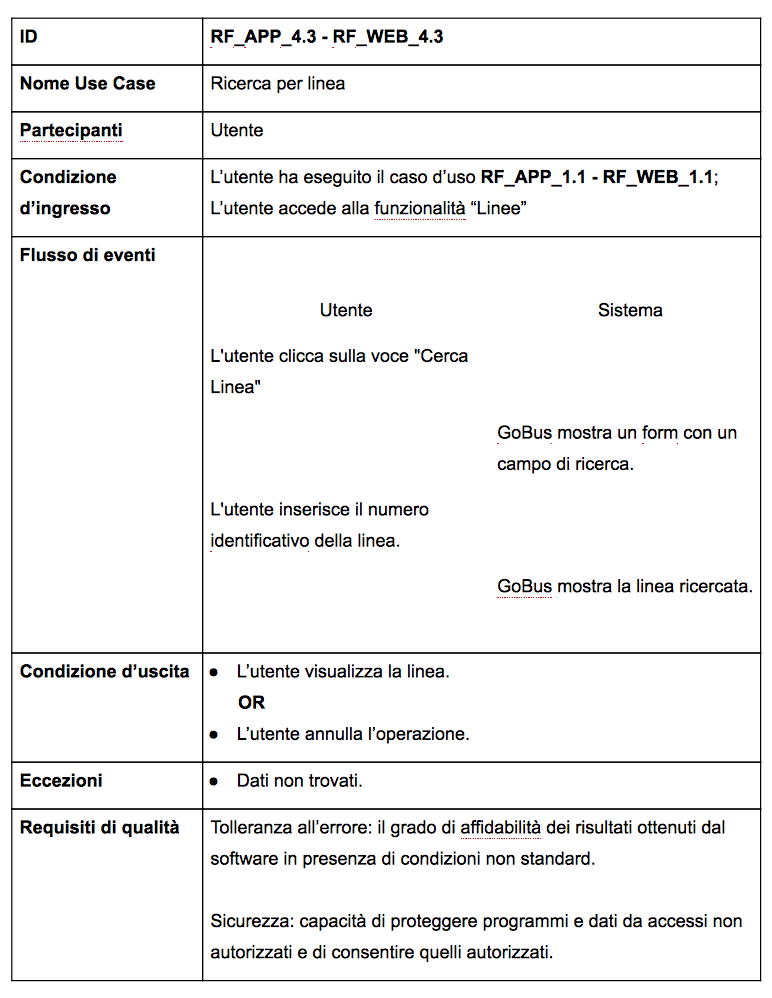
\includegraphics[scale=.7]{img/cd.png}
\caption{Caso d\rq uso relativo al requisito funzionale che consente la ricerca di una linea.}
\label{fig:cd}
\end{figure*}

La Figura \ref{fig:cd} mostra il caso d\rq uso relativo al requisito funzionale che consente la ricerca di una linea. In particolare, l'utente registrato, dopo aver effettuato l'accesso al sistema (condizione d\rq entrata necessaria), clicca sul tasto che consente la ricerca di una linea e digita la query di ricerca prescelta. Il sistema acceder\`{a} all'archivio dati e caricher\`{a} la linea ricercata. Vale la pena notare che ogni caso d\rq uso del sistema modella un requisito sia considerando le azioni che intercorrono tra l\rq utente e il sistema, sia considerando i requisiti di qualit\`{a} ed eventuali condizioni che potrebbero causare eccezioni.\\

Il successivo step nella modellazione delle funzionalit\`{a} del sistema è consistito nella definizione dei path navigazionali relativi a ciascun raggruppamento di requisiti identificato. Di seguito \`{e} mostrato il path navigazionale che consente ad un utente registrato di muoversi all\rq interno della gestione delle linee, di cui il requisito di ricerca delle linee è incluso.

\begin{figure*}[h]
\centering
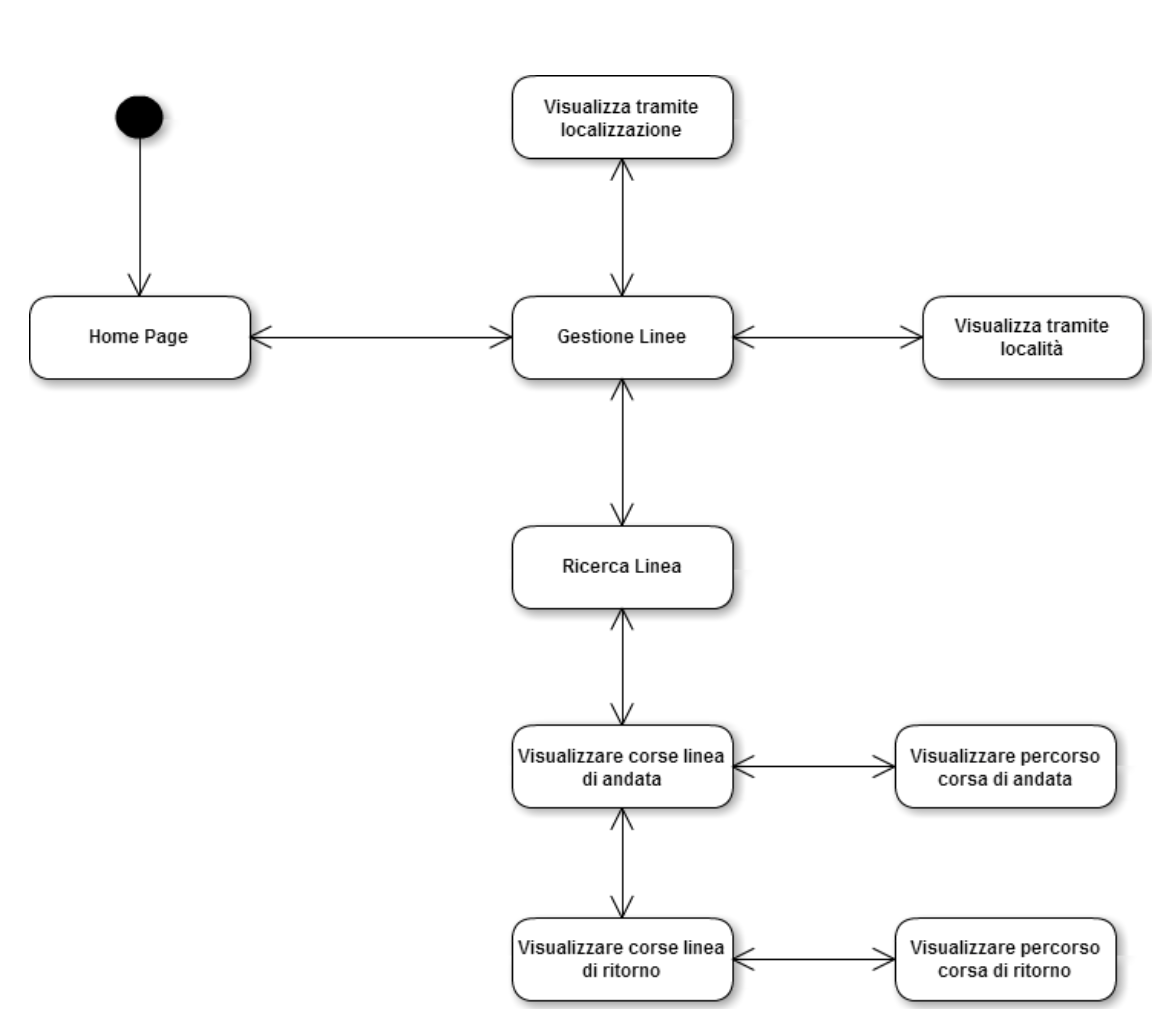
\includegraphics[scale=.9]{img/np.png}
\caption{Path navigazionale relativo alla gestione delle linee.}
\label{fig:np}
\end{figure*} 

Come mostrato in Figura \ref{fig:np}, l'utente, a partire dalla Home Page dell'applicazione, pu\`{o} accedere alla funzionalit\`{a} di Gestione delle Linee, all\rq interno della quale \`{e} data la possibilit\`{a} di accedere i) alla visualizzazione delle linee tramite geo-localizzazione e  ii) visualizzazione della ricerca di una linea. Effettuando il caso d\rq uso mostrato in Figura \ref{fig:cd}, l\rq utente accede alla schermata di visualizzazione delle corse di andata per la linea selezionata, con la possibilit\`{a} di visualizzare anche la corsa di ritorno.\\

Infine, l'ultima parte dell\rq analisi dei requisiti è consistita nella definizione dei mockup delle funzionalit\`{a} identificate. In Figura \ref{fig:ui} \`{e} mostrato il mockup della funzionalit\`{a} di ricerca di una linea, implementato sulla base di una interfaccia per smartphone. 

\begin{figure}[tb]
\centering
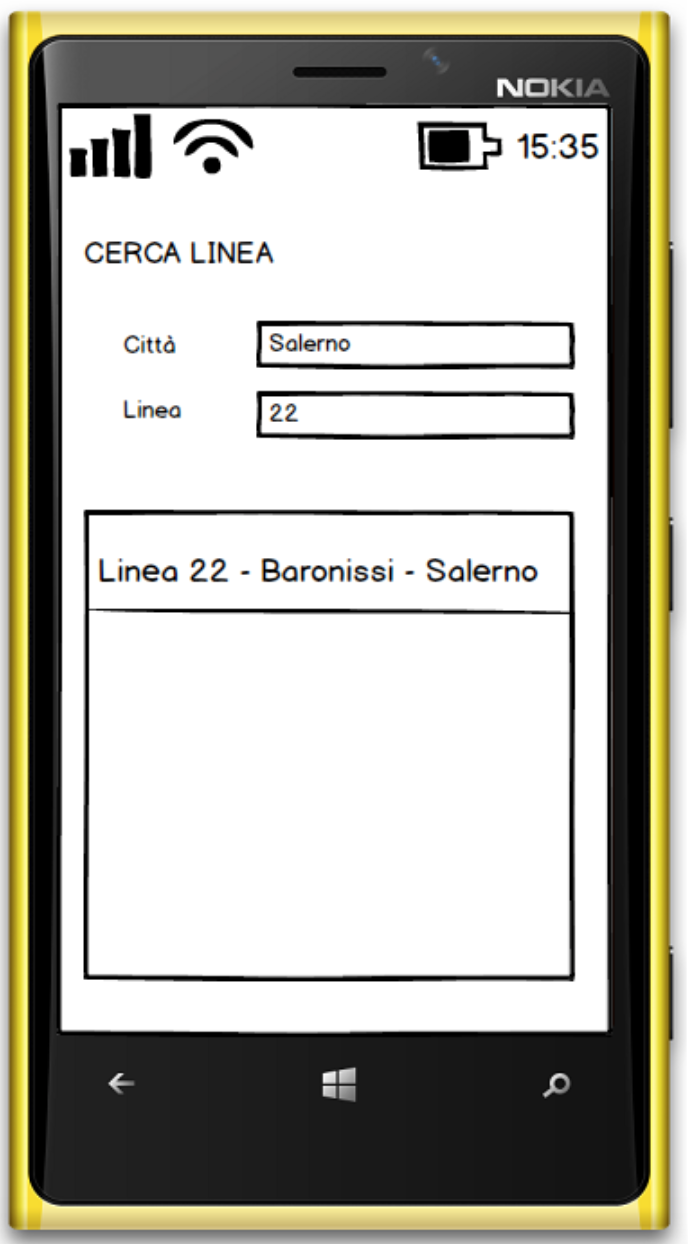
\includegraphics[scale=.3]{img/ui.png}
\caption{Screen Mockup della Funzionalit\`{a} di Ricerca di una Linea.}
\label{fig:ui}
\end{figure} 

La definizione degli screen mockup ci ha aiutato nella comprensione dei requisiti, ma anche nella definizione degli artefatti di basso livello descritti nelle successive sezioni. 

\subsection{Design}
Gli obiettivi principali della fase di design sono stati quelli di definire i) i design goal; ii) l\rq architettura dell\rq applicazione; e iii) il mapping hardware-software. Il primo step \`{e} consistito nella definizione degli obiettivi di design a partire dai requisiti non funzionali presenti nel documento di analisi e specifica dei requisiti. Sono stati identificate 4 categorie di design goal, di seguito riportati:\\

\noindent {\bf{DG-0 - Dependability criteria}}:  \emph{GoBus} garantir\`{a} il corretto svolgimento delle proprie funzioni, gestendo i vari errori logici (quelli derivanti da una negligenza da parte dell’utente), che potranno verificarsi durante l’utilizzo, ed eventuali attacchi alla sicurezza. Questo insieme di design goal comprende i requisiti di robustezza, affidabilit\`{a}, disponibilit\`{a} e sicurezza.\\
\noindent {\bf{DG-1 - Performance criteria}}:  Il sistema sar\`{a} usabile e leggero, in modo tale che, nel caso in cui più persone accedano al sistema contemporaneamente, questo non venga rallentato. In definitiva, il sistema dovr\`{a} garantire che le varie operazioni offerte vengano svolte entro un intervallo di tempo accettabile. Questo insieme di design goal comprende i tempi di risposta, il throughput, e i requisiti di memoria.\\
\noindent {\bf{DG-2 - Maintenance criteria}}:  \emph{GoBus} garantir\`{a} un alto grado di manutenibilit\`{a}. Questo insieme di design goal comprende l\rq estendibilit\`{a}, la modificabilit\`{a} e la tracciabilit\`{a} dei requisiti.\\
\noindent {\bf{DG-3 - End User criteria}}:  \emph{GoBus} garantir\`{a} la learnability e l\rq usabilit\`{a} del sistema.\\

Per quanto riguarda l\rq architettura del sistema, \emph{GoBus} sar\`{a} implementato in una architettura three-tier, e quindi tramite una suddivisione del sistema in tre livelli: i) \emph{presentation-layer}, \emph{application-layer} e \emph{storage-layer}. Il primo livello consiste di tutte le interfacce grafiche che consentiranno all\rq utente di poter dialogare con la logica di business, a sua volta implementata nell\rq application-layer. Infine, lo storage-layer contiene le componenti che consentono l\rq immagazzinamento dei dati.\\

Il successivo passo \`{e} consistito nella decomposizione del sistema in sottosistemi. In questo contesto, le metriche di coesione e accoppiamento rappresentano un importante strumento per poter definire una decomposizione che consenta a team di sviluppo separati di poter eseguire parallelamente diversi task. Nel nostro contesto, \`{e} stata definita la decomposizione mostrata in Figura \ref{fig:sd}.

\ref{fig:sd}
\begin{figure*}[tb]
\centering
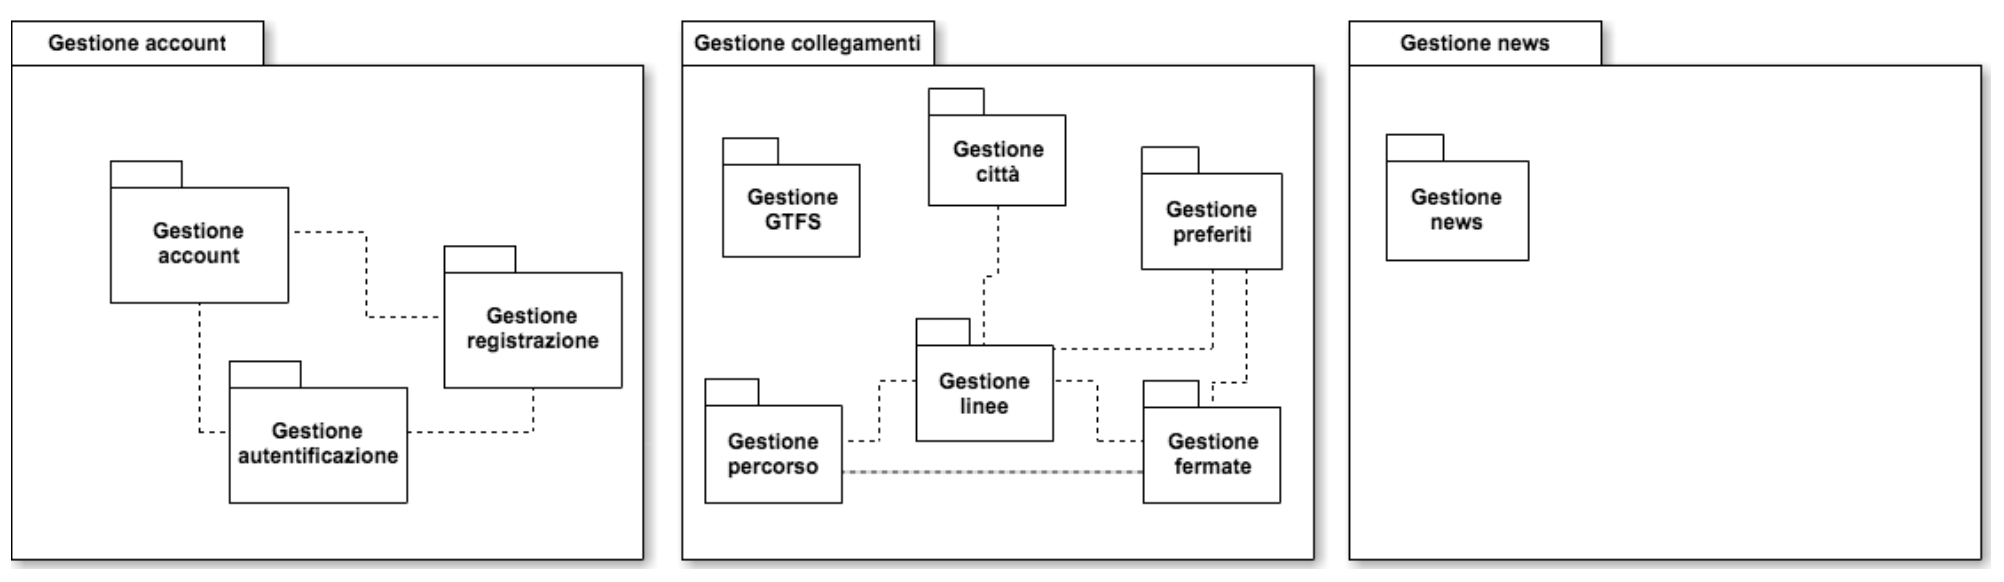
\includegraphics[scale=.4]{img/sd.png}
\caption{Decomposizione in Sottosistemi}
\label{fig:sd}
\end{figure*} 

Come \`{e} possibile vedere, \emph{GoBus} si compone di tre sottosistemi, che fanno riferimento i) alla gestione degli utenti (Gestione Account in Figura \ref{fig:sd}), ii) la gestione di tutti i dati relativi alle fermate, alle linee e ai percorsi (Gestione Collegamenti in Figura \ref{fig:sd}), e iii) la gestione dei preferiti, che rappresenta una componente a se stante nell\rq economia del sistema.\\

\begin{figure*}[tb]
\centering
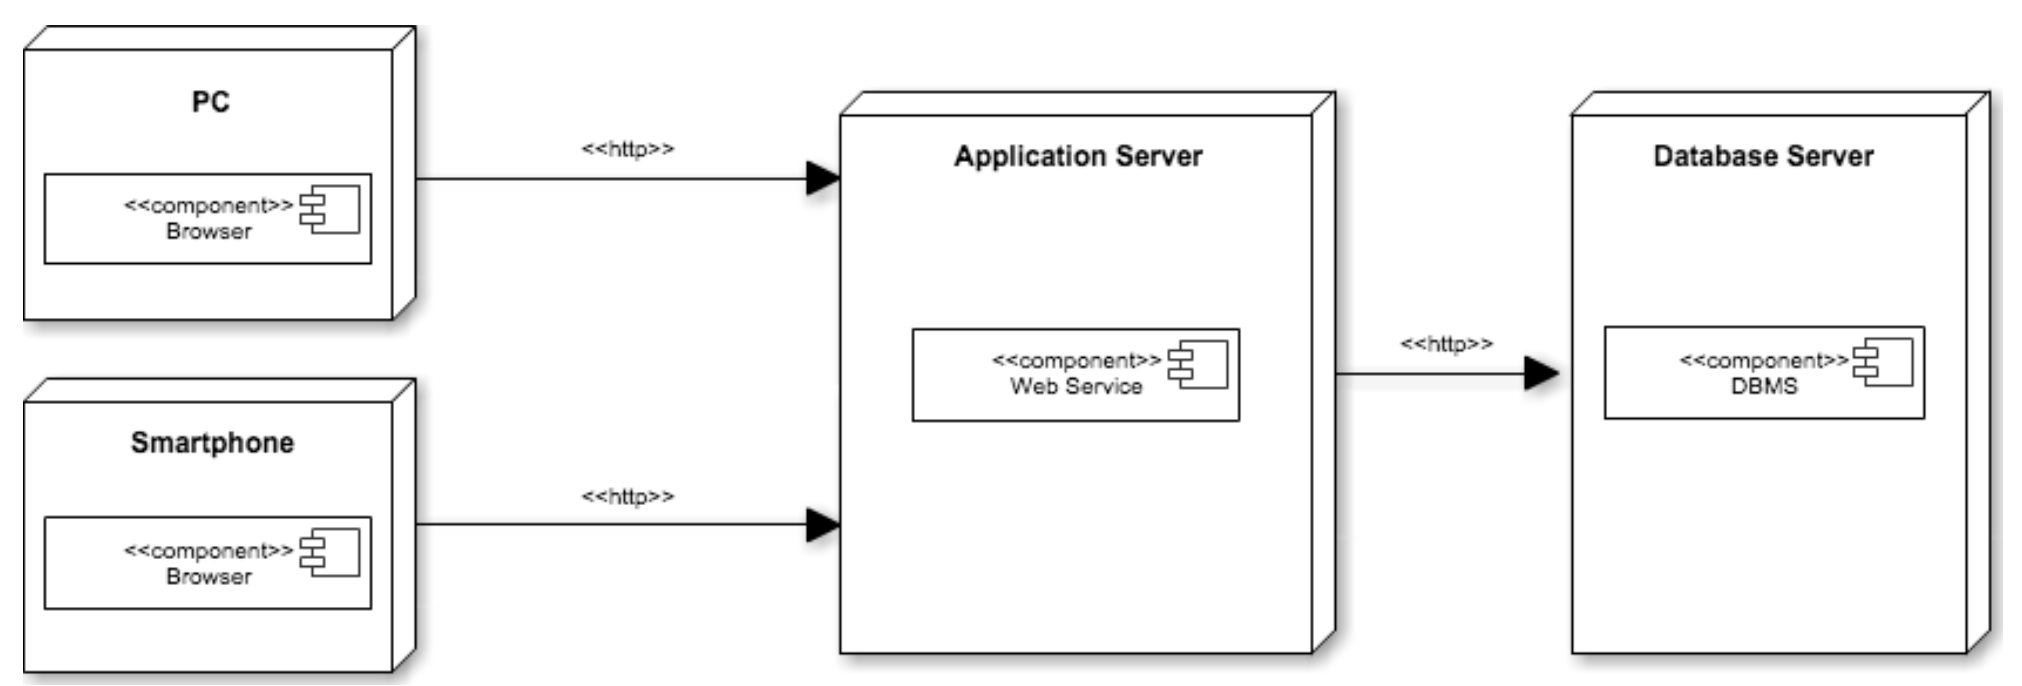
\includegraphics[scale=.4]{img/mhs.png}
\caption{Mapping Hardware/Software}
\label{fig:mhs}
\end{figure*} 

Infine, \`{e} stato definito il mapping hardware-software. Il Deployment Diagram fornisce un ausilio agli sviluppatori per quanto riguarda l\rq organizzazione delle componenti hardware e software del sistema \emph{GoBus}. In figura \ref{fig:mhs} possiamo vedere quali sono i nodi che interagiscono col sistema: Application Server e il Database Server. Le interfacce dei vari sottosistemi accedono ai pacchetti dell\rq Application Server, in cui risiedono gli oggetti di tipo control ed entity. L\rq accesso al database avviene tramite un sottosistema di storage, per garantire, anche, l’indipendenza di esso; infatti se sorgesse la necessit\`{a} di modificare una qualsiasi componente dell’interfaccia del sottosistema, non vi sarebbe il bisogno di apportare innumerevoli modifiche all’interno del sistema. La comunicazione tra i nodi avviene tramite protocollo HTTP.\\
Infine, all\rq interno del design \`{e} stato analizzata la metodologia di mantenimento dei dati persistenti, cos\`{i} come il controllo degli accessi. Il dettaglio completo delle attivit\`{a} svolte in questa fase \`{e} nel documento di System Design allegato.

\subsection{Implementazione}

\subsection{Testing}

\subsection{Rilascio}